\chapter{Grundlagen}
\label{Grundlagen}
Das Ziel dieser Arbeit besteht darin aus einem UML-Modell ein GWT-Projekt zu
generieren. Zur Verständnis werden in diesem Kapitel einige wichtige
Grundlagen erläutert.
% ---------------------------------------------
% MDA
% ---------------------------------------------
\section{Model Driven Architecture} \label{MDA}
Model Driven Architecture (dt. Modellgetriebene Architektur), kurz MDA genannt, stellt
einen bestimmten Ansatz zur Softwareentwicklung dar. Dieses Konzept ist 2001 von der
Object Management Group (OMG) veröffentlicht worden und gilt heute als
Standard. Hierbei werden Richtlinien zur Spezifikation in Form von Modellen vorgegeben.
Aus diesen Modellen, die formal eindeutig sind, wird dann mithilfe von Generatoren
automatisch der benötigte Code erzeugt. Ziel der MDA-Architektur ist es, den gesamten Prozess der Softwareerstellung in möglichst plattformunabhängigen Modellen darzustellen, so dass die Software zu einem hohen Anteil automatisch durch Transformationen von Modellen erzeugt werden kann. Die dabei entstehenden Transformatoren können eine hohen Wiederverwendbarkeit und Wartbarkeit sicher stellen. 
Bei den Modellen handelt es sich im Speziellen, um das Platform Independent Model und das Platform Specific Model, welche bei diesem Projekt auf das Metamodell der UML 2.4 Anwendung fanden. So kann in dieser Arbeit das Profil als PIM verstanden werden, welches dann durch das Klassenmodell (PSM) spezifiziert wurde.
Was dies genau bedeutet und wie die verschiedenen Modelle zu verstehen sind, wird in dem folgenden Abschnitt erläutert

\subsection{Platform Independent Model und Plattform Specific Model} \label{PIMPSM}
Das Platform Independent Model (PIM, dt. Plattformunabhängiges Modell) stellt ein
Softwaresystem dar, das unabhängig von der technologischen Plattform ist. Zudem wird die konkrete technische Umsetzung des Systems nicht berücksichtigt. In dem PIM
sind alle Anforderungen erfasst. Alles, was es zu spezifizieren gibt im System, ist definiert,
jedoch komplett frei von der später folgenden Implementierung. Somit ist nicht nur eine
einzige Implementierung des Systems möglich, sondern durchaus mehrere
unterschiedliche.
Werden nun die Funktionalitäten kombiniert, die im Platform Independent Model definiert sind, mit den Designanforderungen der gewünschten Plattform, so entsteht das Platform Specific Model (PSM, dt. Plattformspezifisches Model). Dies geschieht über Modelltransformationen. Das nun entstandene PSM kann durch weitere Transformationen immer spezifischere Modelle erstellen, bis letztendlich der Quellcode für eine Plattform generiert wird. Im Gegensatz zum PIM, welches nur die
fachlichen Anforderungen definiert, werden beim PSM auch die technischen Aspekte
eingebunden.\cite[S.377 ff.]{bib:MDA2}\cite{bib:MDA3}\\ 
 
Allerdings ist zu beachten, dass es sich bei PIM und PSM um relative Konzepte handelt. 
In diesem Projekt sind sowohl M1 als auch M2 Modell im Bezug auf GWT als PIM zu betrachten. Die eigentliche Spezifizierung für GWT erfolgt erst bei der Model-To-Text Transformation im Generator.
% ---------------------------------------------
% GWT
% ---------------------------------------------
\section{GWT}
\label{GWT}
Das Google Web Toolkit, kurz GWT, ist ein open-source Projekt von Google. Es
dient der Entwicklung von Webanwendungen mittels Java. Dabei übersetzt der GWT
Compiler den gesamten Java Source-Code in JavaScript Code und DOM-Elemente.
Während der Übersetzung des Java Codes zu JavaScript Code werden darüber hinaus Optimierungen vorgenommen wie das Löschen von dead-Code. Dies führt potenziell dazu, dass komplexe
Anwendungen im Browser schneller ausgeführt werden können. Darüber hinaus bietet
GWT noch weitere Möglichkeiten, die dem Entwickler einer Webanwendung zu Gute
kommen. Dazu zählen u. A. das Integrieren von JavaScript Code oder von
JavaScript Bibliotheken innerhalb des Java Codes durch das JavaScript Native
Interface, kurz JSNI und das sogenannte Code-Splitting, welches einem Entwickler
ermöglicht sogenannte Split Points innerhalb des Codes zu setzen, welche dazu
führen, dass bei der Ausführung der Anwendung bestimmte Inhalte ab dem Split
Point später nachgeladen werden und dadurch die Startladezeit verringern.
Google bietet mit zu den genannten Eigenschaften weitere positive
Software Engineering Aspekte. Durch GIN (GWT INjection) 

\subsection{MVP}
\label{MVP}
MVP (Model-View-Presenter) ist ein Design Pattern. Es ist ähnlich dem MVC
(Model-View-Controller). Google beschreibt den Nutzen des MVP Patterns in der
Einbindung von Testfällen in einer GWT Anwendung. Darüber hinaus kann dieses
Pattern auch genutzt werden, um eine GWT Anwendung für verschiedene Plattformen
verfügbar zu machen. Diese Plattformen können z.B. der Browser auf mobilen
Endgeräten oder auf dem Desktop sein.
\begin{figure}[htbp]
\begin{center}
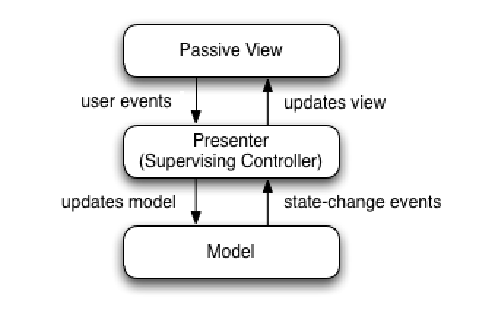
\includegraphics{./img/MVP.pdf}
\caption{Visualisierung des MVP Patterns \cite{bib:MVP1}}\label{Fig:MVP}
\end{center}
\end{figure}\\
Der Presenter übernimmt die Logik und die View ist einfach gehalten
\cite{bib:MVP2}. Dies sorgt für eine klare Trennung zwischen Model und View (vgl.
Abbildung \ref{Fig:MVP}). Bei MVC hingegen kennt die View das Model.
\cite{bib:MVCvsMVP}. Der Presenter steuert die View und übermittelt die Daten
des Model's zur View.
Daher wird der einfache Austausch von Views ermöglicht ohne das weitere
Änderungen vorgenommen werden müssen \cite{bib:MVP1}\cite{bib:MVP2}.

In der zu generierenden Anwendung soll dieses Pattern ohne ein Model
implementiert werden, da der Fokus ausschließlich auf eine GWT Frontend
Anwendung gerichtet ist. Die MVP Struktur ist dabei so umgesetzt, sodass der
Presenter als Interface in dem View Interface und konkret über die Activity
definiert wird. Die Activity regelt zusätzlich das Event Handling und die
Datenbeschaffung. Die View Implementierung beinhaltet eine
Instanz des Presenters, damit die Aktionen der View Komponenten
(bei GWT Widgets genannt) an den Presenter übergeben und dadurch an die
Activity weitergeleitet werden.

\subsection{UiBinder}
\label{UiBinder}
Das UiBinder Framework für GWT Anwendungen ist ähnlich zu betrachten wie HTML
und CSS. Dieses Framework ermöglicht das Layouting von GWT Websites. Dabei
wird die Website nicht nur über den Code erzeugt, sondern zusätzlich mittels
einer xml-Datei, die ui.xml Datei. In dieser Datei können innerhalb eines ui:Style
Tags (vgl. Listing \ref{lst:BSPCodeUIXML}) Style
Eigenschaften ähnlich wie bei CSS gesetzt werden. Dies bietet die Möglichkeit die
View Implementierung zu entkoppeln. Darüber hinaus existieren noch weitere
Möglichkeiten zur Entkopplung der View Implementierung, sodass z.B.
statische View Komponenten nur innerhalb der ui.xml
Datei enthalten sind und somit ein Overload der View Implementierung vermindert
werden kann. Weiterhin können die Komponenten innerhalb dieser Datei gebunden
werden an die Komponenten in der View Implementierung \cite{bib:uiBind}. Dazu
folgender Codeauszug von einem vorangegangenem GWT Projekt zur Erläuterung dieses Zusammenhangs.\\
\lstset{language=gwt}
\begin{lstlisting}[caption={Beispielcode UiBinder in View
Implementierung}, label={lst:BSPCodeView}]
	private static LoginViewImplUiBinder $uiBinder$ = GWT
			.create(LoginViewImplUiBinder.class);

	interface LoginViewImplUiBinder extends 
			UiBinder<Widget, LoginViewImpl> {}

	|@UiField|
	TextBox $name$;
		
	//Constructor
	|@Inject|
	public LoginViewImpl() {
		$content$.add($uiBinder$.createAndBindUi(this));
	}
	|@UiHandler|({ "button" })
	void onButtonPressed(ClickEvent e) {
		// do something
	}
\end{lstlisting}
\lstset{language=uixml}
\begin{lstlisting}[caption={Beispielcode UiBinder in ui.xml},
label={lst:BSPCodeUIXML}]
<!DOCTYPE ui:UiBinder SYSTEM 
	"http://dl.google.com/gwt/DTD/xhtml.ent">
<ui:UiBinder xmlns:ui="urn:ui:com.google.gwt.uibinder"
	xmlns:g="urn:import:com.google.gwt.user.client.ui"
	xmlns:my="urn:import:myprojectpackage">
	<ui:style>
		.enterbutton {
			font-size: 16px;
			font-weight: bold;
			padding: 10px;
			color: #336699;
		}
	</ui:style>
	<g:FlowPanel>
		<g:Label text="Anmeldename"></g:Label>
		<g:TextBox ui:field="name"></g:TextBox>
		<g:Button text="Einloggen" ui:field="button" 
			styleName="{style.enterbutton}"></g:Button>
	</g:FlowPanel> 
</ui:UiBinder> 
\end{lstlisting}
Die Annotationen @UiField und @UiHandler in der View Implementierung (vgl.
Listing \ref{lst:BSPCodeView}) ermöglichen den Zugriff auf die View Komponenten
mit dem jeweiligem Attribut ui:field in der ui.xml (vgl. Listing
\ref{lst:BSPCodeUIXML}). @UiField ist dabei dafür zuständig die Instanz zu
erhalten. Diese kann dann z.B. über den Java Code definiert oder Style
Eigenschaften gesetzt werden. Entgegen dem ermöglicht @UiHandler die Anmeldung
einer Methode auf der Instanz. Darüber kann dann im Falle des Beispiels ein
Klick Event auf dem Button ausgeführt werden.

Damit zeigen die Listings \ref{lst:BSPCodeView} und \ref{lst:BSPCodeUIXML}
nur kleine Beispiele für die Nutzung von dem UiBinder Framework, welche
innerhalb des Generator Projektes umgesetzt werden sollen.




% ---------------------------------------------
% GIN
% ---------------------------------------------
\section{Dependency Injection mittels GIN}
\label{GIN}